% !TeX program = xelatex
% ↑ Automatische Auswahl für XeLaTeX compiler

% Das ist mein Template für die TX000 Arbeiten. Nicht perfekt, also falls ihr Verbesserungsvorschläge habt, stellt gerne einen Pull-Request. https://github.com/NikomitK/TX000_Template
% Bitte lasst auch einen star auf github da, danke.
% Wenn ihr die cite funktion von LaTeX nutzen wollt, müsst ihr einfach die Quellen im bibtex Format in die sources.bib datei kopieren, google scholar z.B. hat bei den Quellen einen Button mit dem man das so bekommt, auch viele andere websites.
% Bilder kommen in den images Ordner, den müsst ihr beim abrufen eines Bildes nicht angeben, passiert automatisch.


% Trag hier deine Daten ein, die entsprechenden Felder werden automatisch angepasst.
\def\meinTitel{Verteilte Systeme: Filesharing-Plattform}
\def\artDerArbeit{Ausarbeitung}
\def\meinName{Aziz Carducci, Sven Sendke}
\def\meinKurs{TINF22F}
\def\meineMatrikelNr{1965015, 8469950}
\def\firmenName{Allianz Lebensversicherungs-AG}
\def\projektBetreuer{Benjamin Salchow}
\def\abgabeDatum{16.12.2024}
%-----------------------------------------------------------------------------------


\documentclass[12pt]{report}
\usepackage[heightrounded]{geometry}
\geometry{
	a4paper,
	lmargin=3.1cm, %Seitenrand left
	tmargin=2.8cm, %Seitenrad top
	headsep=35pt %Abstand von Kopfzeile
}
\usepackage[onehalfspacing]{setspace}
\usepackage[compact]{titlesec}
\usepackage{cite} % Zitierungen
\usepackage{struktex} % Struktogramme
\usepackage{array} % kp hat chatgpt benutzt
\usepackage{longtable} % Tabelle über einen seitenumbruch
\usepackage[nohyperlinks, printonlyused]{acronym} % abkürzungsverzeichnis
\usepackage{fontspec}
\usepackage{blindtext} % LoremIpsum
\usepackage{fancyhdr} % Kopf- und Fußzeile
\usepackage[export]{adjustbox} % Bilder alignment
\usepackage{stfloats} % Tabular at bottom
%\usepackage[table]{xcolor} %Tabellen farben
\usepackage{tabularx} % Anpassbarere tabellen
\usepackage{easyReview} % Review anmerkungen

\usepackage[utf8]{inputenc} % this is needed for umlauts
\usepackage[ngerman]{babel} % this is needed for umlauts
\usepackage[T1]{fontenc}    % this is needed for correct output of umlauts in pdf


\usepackage{subcaption} % Für subfigures glaub


\usepackage{tikz} % Zum zeichnen
\usetikzlibrary{calc}
\usetikzlibrary{shapes.geometric, arrows}
\setmainfont[Scale=1.1]{Arial}

%--------------------Flowcharts--------------------
\tikzstyle{startstop} = [rectangle, rounded corners, minimum width=3cm, minimum height=1cm,text centered, draw=black, fill=red!30]
\tikzstyle{io} = [trapezium, trapezium left angle=70, trapezium right angle=110, minimum width=3cm, minimum height=1cm, text centered, draw=black, fill=blue!30]
\tikzstyle{process} = [rectangle, minimum width=3cm, minimum height=1cm, text centered, draw=black, fill=orange!30]
\tikzstyle{decision} = [diamond, minimum width=3cm, minimum height=1cm, text centered, draw=black, fill=green!30]
\tikzstyle{arrow} = [thick,->,>=stealth]
%--------------------------------------------------


%--------------------Codeblöcke--------------------
\usepackage{listings} %Für Codeblöcke
\usepackage{color} %Farben für Codeblöcke?
\definecolor{dkgreen}{rgb}{0,0.6,0}
\definecolor{gray}{rgb}{0.5,0.5,0.5}
\definecolor{mauve}{rgb}{0.58,0,0.82}

\lstset{
	language=Java,
	aboveskip=3mm,
	belowskip=3mm,
	showstringspaces=false,
	columns=flexible,
	basicstyle={\small\ttfamily},
	numbers=none,
	numberstyle=\tiny\color{gray},
	keywordstyle=\color{blue},
	commentstyle=\color{dkgreen},
	stringstyle=\color{mauve},
	breaklines=true,
	breakatwhitespace=true,
	tabsize=3
}
%-------------------------------------------------

\usepackage{graphicx} %Package für Bilder
\graphicspath{ {./images/} } %Ordner für Bilder

\sloppy % damit lange Wörter nicht über die Zeile hinausgeschrieben werden.

%--------------------Chapter Heading--------------------
\makeatletter
\def\@makechapterhead#1{%
	\vspace*{-20\p@}%
	{\parindent \z@ \raggedright \normalfont
		\ifnum \c@secnumdepth >\m@ne
		%\huge\bfseries \@chapapp\space \thechapter
		\Huge\bfseries \thechapter.\space%
		%\par\nobreak
		%\vskip 20\p@
		\fi
		\interlinepenalty\@M
		\Huge \bfseries #1\par\nobreak
		\vskip 20\p@
}}
\makeatother
\makeatletter
\def\@makeschapterhead#1{%
	\vspace*{-20\p@}%
	{\parindent \z@ \raggedright \normalfont
		%\huge\bfseries \@chapapp\space \thechapter
		\Huge\bfseries\space%
		%\par\nobreak
		%\vskip 20\p@
		\interlinepenalty\@M
		\Huge \bfseries #1\par\nobreak
		\vskip 20\p@
}}
\makeatother
%-------------------------------------------------------

%\addto\captionsngerman{\renewcommand{\listfigurename}{}}
 % titel von abbildungsverzeichnis weg?

\setlength\parindent{0pt} %Auto Einrücken deaktivieren


%-------------Setup für Inhaltsverzeichnis--------------
\renewcommand{\contentsname}{Inhaltsverzeichnis} %Umbenennung TOC

\usepackage{tocloft} % Formatierung TOX

\setlength{\cftbeforetoctitleskip}{0pt}

\setlength{\cftsubsecnumwidth}{4em} %abstand kapitelnummer - titel

\renewcommand{\cfttoctitlefont}{\huge\bfseries}
\renewcommand{\cftloftitlefont}{\huge\bfseries}

\renewcommand\cftchapfont{\Large\bfseries}
\renewcommand\cftchappagefont{\large}

\renewcommand\cftsecfont{\large\bfseries}
\renewcommand\cftsecpagefont{\large}

\renewcommand\cftsubsecfont{\large}
\renewcommand\cftsubsecpagefont{\large}

\renewcommand\cftsubsubsecfont{\normalsize}
\renewcommand\cftsubsubsecpagefont{\normalsize}


\renewcommand\cftchapafterpnum{\par\addvspace{8pt}}
\renewcommand\cftsecafterpnum{\par\addvspace{8pt}}
\renewcommand\cftsubsecafterpnum{\par\addvspace{6pt}}
\renewcommand\cftsubsubsecafterpnum{\par\addvspace{6pt}}
%-------------------------------------------------------


%------------------Setup für LoF/LoT--------------------
\makeatletter
\renewcommand{\@cftmakeloftitle}{}
\renewcommand{\@cftmakelottitle}{}
\makeatother
\setlength{\cftfigindent}{0em} % change indentation of e.g. "Figure 1" within list of figures
\renewcommand\cftfigfont{\large}
\renewcommand\cftfigpagefont{\large}
\setlength{\cfttabindent}{0em} % change indentation of e.g. "Figure 1" within list of figures
\renewcommand\cfttabfont{\large}
\renewcommand\cfttabpagefont{\large}
\setlength{\cftbeforeloftitleskip}{0pt}
\setlength{\cftbeforelottitleskip}{0pt}
%-------------------------------------------------------


%----------------Setup für Verlinkungen-----------------
\usepackage{hyperref}
\hypersetup{
	colorlinks,
	citecolor=black,
	filecolor=black,
	linkcolor=black,
	urlcolor=black
}
%-------------------------------------------------------


%-------------Kopf-/Fußzeile für Titlepage--------------
\fancypagestyle{titlepage}
{
	\fancyhead[L]{
\includegraphics[scale=0.09]{firmenlogo}}
	\fancyhead[R]{
\includegraphics[scale=0.25]{dhbw}}
	\renewcommand{\headrulewidth}{0pt}
	\fancyfoot[C]{}
}
%-------------------------------------------------------

\begin{document} 
	
	\begin{titlepage}
		\thispagestyle{titlepage}
		\newcommand\HRule{\rule{\textwidth}{1pt}} %Titellinien
		
		
		\begin{center}
			
			\vspace*{2cm}
			
			%Title
			\begin{spacing}{2}
				{ \huge \bfseries \MakeUppercase{\meinTitel}}
				%{ \large \bfseries subTitle}\\[0.4cm]
			\end{spacing}
			
			\vspace*{1.5cm}
			
			%Art der Arbeit
			\Large \artDerArbeit
			
			\vspace*{2cm}
			
			%Hochschule
			{\LARGE Studiengang Informatik}\\
			{\LARGE an der Dualen Hochschule}\\
			{\LARGE Baden-Württemberg Stuttgart}\\
			
			\vspace*{2cm}
			
			\Large von \meinName
			
			\vspace*{1.5cm}
			
			\Large Abgabedatum: \abgabeDatum
			
			\begin{table*}[bp]
				\centering
				\begin{tabular}{l l}
					Kurs: & \meinKurs  \\
					Matrikelnummer: & \meineMatrikelNr  \\
					Unternehmen: & \firmenName \\
					Projektbetreuer: &  \projektBetreuer\\
				\end{tabular}
			\end{table*}
			
			
		\end{center}
		
	\end{titlepage}


%------------------Kopf- und Fußzeile-------------------
\fancypagestyle{plain}{
	\fancyfoot[L]{\meinName\\
		 \meinKurs}
	\fancyfoot[C]{Seite \thepage\ }% von \pageref{LastPage}}
	\fancyfoot[R]{\abgabeDatum}
}

\pagestyle{plain}
\fancyhead{}


\fancyhead[L]{
\includegraphics[scale=0.09]{firmenlogo}}
\fancyhead[C]{\nouppercase\leftmark}
\fancyhead[R]{
\includegraphics[scale=0.25]{dhbw}}

\renewcommand{\footrulewidth}{0.4pt} %Linie für Fußzeile


\renewcommand{\sectionmark}[1]{\markboth{#1}{}} 
%-------------------------------------------------------

\pagenumbering{Roman}
\newpage

%------------------Inhaltsverzeichnis-------------------

\addcontentsline{toc}{chapter}{\protect\numberline{}Inhaltsverzeichnis}
\tableofcontents
\addtocontents{toc}{}
\thispagestyle{plain}

%********************************
%Abbildungsverzeichnis
%********************************
\newpage
\chapter*{Abbildungsverzeichnis}
\addcontentsline{toc}{chapter}{\protect\numberline{}Abbildungsverzeichnis}

\listoffigures

%********************************
%Tabellenverzeichnis
%********************************
\newpage
\chapter*{Tabellenverzeichnis}
\addcontentsline{toc}{chapter}{\protect\numberline{}Tabellenverzeichnis}

\listoftables

\newpage
\chapter*{Abkürzungsverzeichnis}
\addcontentsline{toc}{chapter}{\protect\numberline{}Abkürzungsverzeichnis}
\markboth{Abkürzungsverzeichnis}{Abkürzungsverzeichnis} %Benötigt, damit das im header steht

%********************************
%Abkürzungsverzeichnis
%********************************
\begin{acronym}[SOAP]
	\acro{BA}{Beispiel Acronym}
\end{acronym}


%Speichern des page counters, um bei Literaturverzeichnis weiter zu zählen.
\newcounter{frontmatterPage}
\addtocounter{frontmatterPage}{\value{page}} 

\newpage
\pagenumbering{arabic}
\chapter{Architektur}
	Im Folgenden wird die Architektur im Allgemeinen mit den Systemkomponenten und den Anforderungen dargestellt.
	\section{Allgemein}
		Zuerst betrachten wir die Struktur der Architektur und dann die Architectual Desicion.
		\subsection{Aufbau}
			Die Abbildung \ref{fig:architektur} zeigt die Gesamtarchitektur. Auf die einzelnen Aspekte wird in den folgenden Punkten eingegangen.
			\begin{figure}[h]
				\centering
				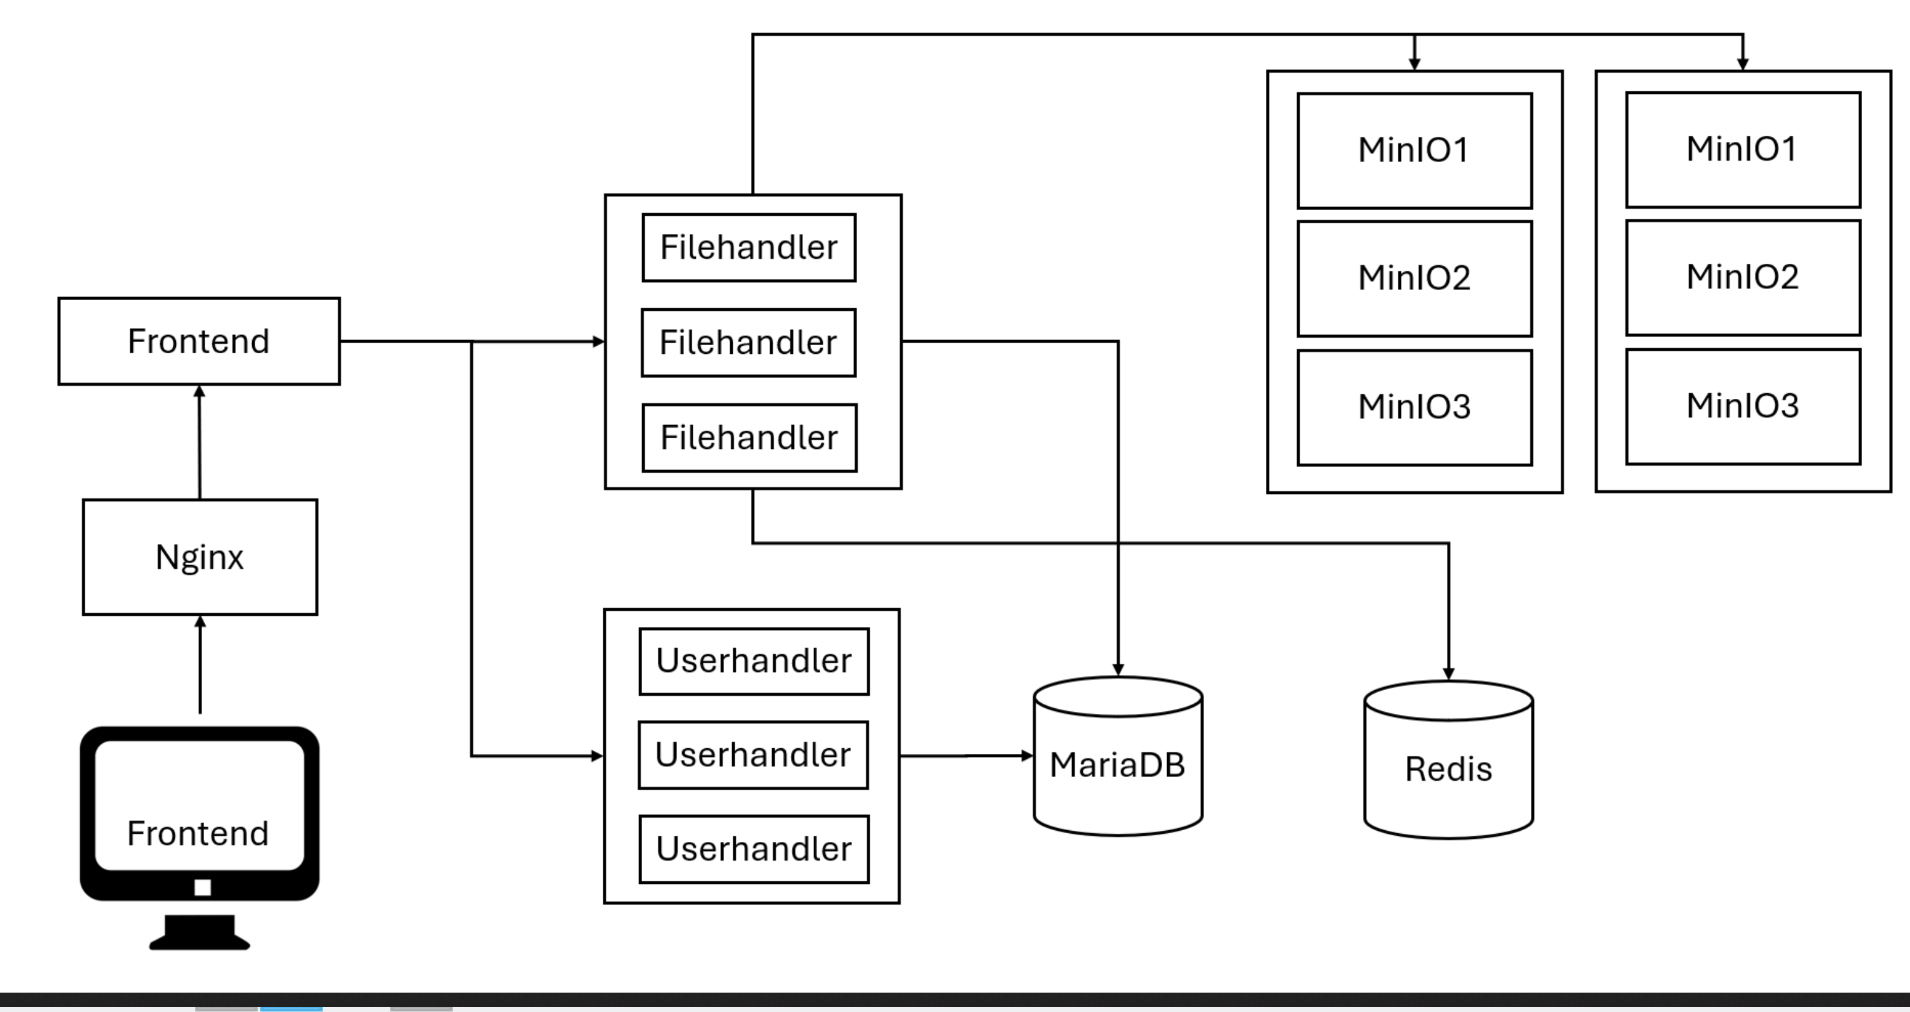
\includegraphics[width=\linewidth]{architektur}
				\caption{Architektur}
				\label{fig:architektur}
			\end{figure}
			
		\subsection{Architectual Decision}
			Folgende Architectual Decision wurden getroffen.
			
			\subsubsection{Microservice-Architektur}
			Die Entscheidung für eine Microservice-Architektur wurde getroffen, um die Modularisierung des Systems zu fördern. Durch die Aufteilung in einzelne, voneinander unabhängige Komponenten wird eine flexible Skalierung ermöglicht, wobei beispielsweise der Filehandler stärker skaliert werden kann als der Userhandler. Zudem erhöht diese Architektur die Ausfallsicherheit, da fehlerhafte Microservices schnell neugestartet werden können, ohne das gesamte System zu beeinträchtigen \cite{taibi2017processes}. Ein weiterer zentraler Vorteil ist die hohe Wartbarkeit: Die Aufteilung in unabhängige, selbstständig deploybare Services erleichtert es Entwicklerteams, Änderungen und Tests durchzuführen, ohne andere Teile des Systems zu beeinflussen, was die verteilte Entwicklung vereinfacht \cite{de2019monolithic}.
			
			\subsubsection{MinIO}
			MinIO wurde als Objektspeicherlösung gewählt, da es die Hochleistungsanforderungen moderner Big-Data-Anwendungen erfüllt \cite{makris2022performiance}. MinIO bietet sowohl bei Lese- als auch bei Schreiboperationen eine herausragende Leistung \cite{makris2022performance}. Wir haben uns für eine S3-Kompatible Objektspeicher-Server entschieden, weil es eine der weit verbreitesten Objektspeicherungs Platforme ist und welche auch Sehr gut dokumentiert ist, aber unteranderem auch da es bei sehr vielen großen Unternehmen genutzt wird und wir diese Erfahrung mitnehmen wollten, da das sehr Praxis bezogen ist.
			
			\subsubsection{Spring Boot}
			Das Spring Boot Framework ist der De-facto-Standard für Java-Microservice-Architekturen. Es zeichnet sich durch seine Fähigkeit aus, enorme Datenmengen zu verarbeiten, was es besonders für die Big-Data-Industrie attraktiv macht \cite{mythily2022analysis}. Darüber hinaus erleichtert Spring Boot die Entwicklung von RESTful-Webservices und APIs erheblich, wodurch Entwickler ihre Aufgaben schneller und effizienter erledigen können \cite{mythily2022analysis}.
			
			\subsubsection{Relationale Datenbank}
			Der Vorteil der relationalen Datenbank besteht darin, dass sie eine solide Grundlage für die Behandlung von Redundanz und Konsistenz von Beziehungen bietet. \cite{codd1970relational}. Dies ist wichtig, um die Daten der Dateien konsistent zu halten. 
			
	\section{Systemkomponenten}
		Im Folgenden wird die Lösung mit ihren Komponenten und deren Interaktion dargestellt.
		\subsection{Komponenten}
			\begin{itemize}
				\item Frontend (Angular): Angular erleichtert sowohl das Routing durch Angular Router als auch REST durch den Angular Service HttpClient.
				\item Filehandler (Spring Boot): Dieser Microservice kümmert sich um die Benutzerregistrierung und -anmeldung und stellt den JWT bereit.
				\item Userhandler (Spring Boot): Dieser Microservice kümmert sich um alle Funktionen, die mit Dateien zu tun haben.
				\item Datenbank (MariaDB):  Speichert Benutzer, Datei-Metadaten und begonnene Konversationen zwischen 2 Benutzern. Das ERM der Datenbank ist in Abbildung \ref{fig:erm} dargestellt.
				\item Redis: Dient als Cache für den Filehandler, mehr dazu später.
				\item Objektspeicherung (MinIO): Drei Minio Instanzen befinden sich in einem Shard. In einem Shard speichern sie dasselbe, aber ansonsten wechseln sie zwischen den Shards, um die Datei zu speichern.
				\item Loadbalancer (Nginx): Verteilt alle Anfragen des Benutzers.
			\end{itemize}
						
			\begin{figure}[h]
				\centering
				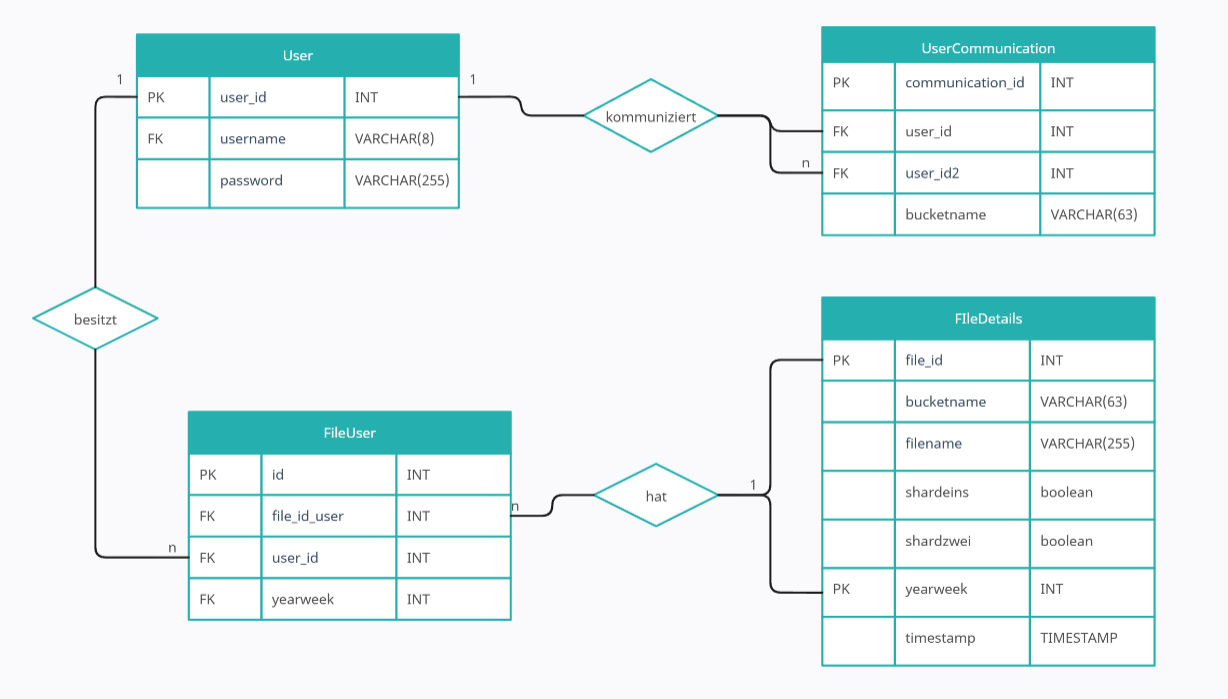
\includegraphics[width=\linewidth]{erm}
				\caption{ERM}
				\label{fig:erm}
			\end{figure}
			
		\subsection{Interaktion Komponenten}
			Die Interaktion zwischen den Komponenten ist in den folgenden Sequenzdiagrammen dargestellt, wobei die Upload-Funktion in Abbildung \ref{fig:download_sequenz_diagramm} und die anderen Funktionen wie Benutzerregistrierung und -anmeldung , Bucket-Erstellung, Löschen/Download von Dateien in Abbildung \ref{fig:rest_sequenz_diagramm} dargestellt sind. Die Entscheidung Upload-File einzeln darzustellen, war weil es unsere Hauptfunktion ist, wo auch am meisten passiert.
			
			\begin{figure}[h]
				\centering
				\includegraphics[width=0.95\linewidth]{download\_sequenz\_diagramm}
				\caption{Sequenz Diagramm für Download}
				\label{fig:download_sequenz_diagramm}
			\end{figure}
			
			\begin{figure}[h]
				\centering
				\includegraphics[width=0.95\linewidth]{rest\_sequenz\_diagramm}
				\caption{Sequenz Diagramm für restliche Funktionen}
				\label{fig:rest_sequenz_diagramm}
			\end{figure}
		
	\section{Anforderungen}
		Im folgenden sind die Funktionalen sowie die Nichtfunktionalen Anforderungen aufgelistet.
		\subsection{Funktional}
			\begin{itemize}
				\item \textbf{Datei-Upload}: Benutzer können Dateien in verschiedenen Formaten über eine Benutzeroberfläche oder API hochladen.
				\item \textbf{Tauschpartner}: Benutzer können einen anderen Benutzer hinzufügen und Dateien untereinander austauschen.
				\item \textbf{Load Balancing}: Das System verteilt eingehende Uploads und Anfragen automatisch auf verfügbare Server, um eine gleichmäßige Auslastung sicherzustellen.
				\item \textbf{Speicherung im Object Storage}: Dateien werden in einem verteilten Object-Storage-System gespeichert, das hohe Skalierbarkeit und Zuverlässigkeit bietet.
			\end{itemize}
		\subsection{Nichtfunktional}
			\begin{itemize}
				\item \textbf{Skalierbarkeit}: Das System muss in der Lage sein, mit einer wachsenden Anzahl von Benutzern und Dateien ohne Leistungseinbußen zu skalieren.
				\item \textbf{Kompatibilität}: Die Plattform muss mit gängigen Betriebssystemen (Windows, macOS, Linux) und Browsern kompatibel sein.
			\end{itemize}

\chapter{Umsetzung}
	Im Folgenden werden die Umsetzung und mögliche Alternativen dargestellt.
	\section{Implementierung}
		Bei der Implementierung schauen wir uns an, wie diese umgesetzt wurde und welche Schwierigkeiten es dabei gab und wie sie gelöst wurden.
		\subsection{Wie wird die Architektur umgesetzt?}
			\subsubsection{Docker Compose}
				Die Architektur wird mit Docker Compose erstellt. Das Frontend, die Microservices, die Datenbank, der Loadbalancer, Redis und die Shards mit den MinIO-Instanzen werden mit den entsprechenden Dockerfiles gebaut. Die sich daraus ergebende Shard-Struktur ist in Abbildung \ref{fig:shards} dargestellt. Wie zu sehen ist, wird das Prinzip mit 2k+1 für die Ausfallsicherheit eingehalten, auch werden in unserem Beispiel jeweils drei Microservices gestartet.
		
				\begin{figure}[h]
					\centering
					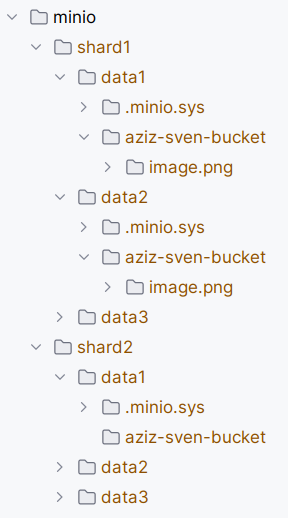
\includegraphics[width=0.8\linewidth]{shards}
					\caption{Shards}
					\label{fig:shards}
				\end{figure}
			
			\subsubsection{Partitionierung}
				Wir haben die horizontale Partitionierung in unserem Projekt implementiert, um die Datenbank effizienter zu gestalten. Dabei teilen wir die Daten wöchentlich auf, sodass jede Woche ihre eigene Partition hat. Das hat den Vorteil, dass bei Abfragen nur die relevanten Daten für die angeforderte Woche geladen werden müssen, was die Abfragegeschwindigkeit verbessert und die Gesamtzahl der Lesevorgänge verringert. Dies sorgt für eine bessere Performance, besonders bei einem skalierten Projekt, da durch das Partnersystem, können bis zu Hunderte von Files pro Woche geschickt werden was schnell dazu sorgt das die Datenbank, sehr voll wird.
				\begin{figure}[h]
					\centering
					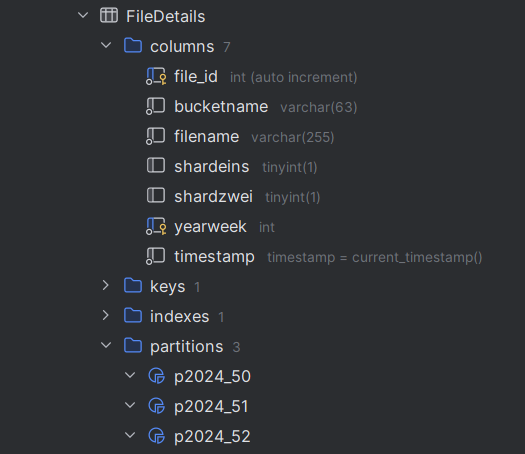
\includegraphics[width=0.8\linewidth]{partitionierung}
					\caption{Partitionierung}
					\label{fig:partitionierung}
				\end{figure}
				
			\subsubsection{Redis}
				Die Implementierung von Redis ermöglicht eine globale, persistente Speicherung des Round-Robin-Zählers, der über verschiedene Backend-Instanzen unseres Services hinweg synchronisiert wird. Dies sorgt für Konsistenz bei der Verteilung der Last auf die Minio-Server und verbessert gleichzeitig die Skalierbarkeit und Fehlertoleranz deiner Anwendung. Weil hierdurch kann ein globaler Round-Robin Service funktionieren, falls mehr als ein Server Aktiv ist.
			\subsubsection{Buckets}
				Das Ziel war nicht, ein Dropbox-ähnliches Filesharing-System zu schaffen, da bei einem solchen Ansatz lediglich ein einziges Bucket benötigt wird, in dem alle Dateien abgelegt werden. Auch wenn dies technisch möglich wäre, wäre es eine einfachere Lösung. Stattdessen wollten wir uns intensiver mit der Funktionsweise von Buckets und dem S3-Modell auseinandersetzen. Daher haben wir entschieden, dass zwei Benutzer sich gegenseitig hinzufügen können und ein separates Bucket für den Austausch ihrer Dateien erstellt wird, sodass die Dateien nur für diese beiden zugänglich sind. Hierbei konnten wir uns nicht nur genauer mit dem kreeieren von Buckets beschäftigen sondern, auch eine Verbindung zwischen einzelne Files und den Buckets erschaffen.
			\subsection{Schwierigkeiten}
				Folgenden Schwierigkeiten haben Stattgefunden und wie sie gelöst wurden.
				
				\subsubsection{Loadbalacing}
					Die erste Schwierigkeit war das Loadbalancen von den MinIO instanzen, hierbei war es schwierig die einzelnen MinIO-Instanzen Instanzen über nginx kommunizieren zu lassen, dies wurde gelöst in dem die MinIO Instanzen jetzt direkt auf einander zugreifen, durch das Driver System.
			
				\subsubsection{Schardaustausch}
					Die zweite Schwierigkeit war der Austausch zwischen den beide Shards. Denn es kam zu Fehler mitunter den Loadbalancen. Um zu wissen auf welchen Shard gespeichert werden muss, musste einen Counter implementiert werden, hierbei war aber das Problem das jede Backend-Instanz ein eigenen Counter initialisiert hat, um das zu lösen wurde mit Redis, der Counter im Cache gespeichert.
				
				\subsubsection{Buckets zwischen zwei Benutzer}
					Die dritte Schwierigkeit war, dass wir entschieden haben, dass zwei Benutzer miteinander privat austaushen können. Bei einen einfachen Plattform wo es nur ein Bucket gibt wie Dropbox muss man nicht spezifische Buckets kreieren für 2 Benutzer. Bei Bucket kreieren muss man auf Namen achten, man darf ihn nur maximal 63 Zeichen geben. Um das zu lösen haben wir check Frontend und Backend Benutzername Maximal 8 Zeichen. und Bucketname ist user1-user2-bucket.
			
	\section{Mögliche Alternativen}
		Obwohl es natürlich Alternativen in der Programmierung gibt, wie z.B. weniger oder mehr Metadaten für die verschiedenen benötigten Informationen zu speichern, wäre eine Alternative in größerem Umfang andere Open Source S3-kompatible Software wie Ceph oder GlusterFS zu verwenden. Anstelle von S3 könnte auch Hadoop HDFS (Hadoop Distributed File System) verwendet werden. Dies ist ebenfalls ein weit verbreitetes verteiltes Dateisystem, wird aber mehr im Bereich Big Data und Analytics eingesetzt. ist aber im Gegensatz zu den anderen nicht S3-kompatibel.
	
\chapter{Reflektion}
	Die folgenden Überlegungen zeigen, was wir anders machen können und was die größten Herausforderungen und ihre Lösungen sind.
	
	\section{Was kann man anders machen?}
	Ein entscheidender Lernpunkt während der Entwicklung war das Datenbanksystem. Rückblickend wäre es sinnvoll gewesen, dieses von Anfang an korrekt zu konzipieren und aufzusetzen. Stattdessen mussten wir es mehrfach anpassen und nachbessern, bis es schließlich wie gewünscht funktionierte. Besonders wichtig wäre es gewesen, von Beginn an auf Skalierbarkeit und die Einhaltung etablierter Konventionen zu achten. Dies hätte nicht nur spätere Komplikationen vermieden, sondern auch die Integration und Wartung des Systems erheblich erleichtert. Dieser Aspekt unterstreicht, wie entscheidend ein solides Fundament bei der Entwicklung komplexer Systeme ist.
	
	\section{Größten Herausforderungen und ihre Lösung}
	Die größte Herausforderung lag in der Koordination und Integration der verschiedenen Systemkomponenten, insbesondere der Shards mit den MinIO-Instanzen, der Datenbank und dem Loadbalancer. Anfangs scheiterte die Kommunikation zwischen den Instanzen, was dazu führte, dass Dateien nicht korrekt gespeichert oder geladen wurden. Dieses Problem lösten wir durch die Einführung eines zweistufigen Shard-Systems, bei dem jeweils drei MinIO-Instanzen innerhalb eines Shards die gleichen Daten speichern. Dieses Redundanzkonzept gewährleistet die Ausfallsicherheit und ermöglicht den reibungslosen Betrieb, selbst wenn eine Instanz ausfällt.
	
	Ein weiteres Problem bestand im Austausch zwischen den beiden Shards. Hier traten Fehler auf, die durch inkorrekte Loadbalancing-Mechanismen verursacht wurden. Um zu bestimmen, welcher Shard für die Speicherung verwendet werden sollte, führten wir einen Zähler ein, der mit Redis implementiert wurde. Redis diente dabei als schneller und zuverlässiger Speicher für den aktuellen Status des Counters.

%********************************
%Literaturverzeichnis
%********************************
\newpage
\pagenumbering{Roman}
\setcounter{page}{\value{frontmatterPage}} %Bei \pagenumbering wird Seitenzähler zurückgesetzt, hier wird der gespeicherte Wert vom frontmatter weitergeführt
\addtocounter{page}{1}
\addcontentsline{toc}{chapter}{\protect\numberline{}Literaturverzeichnis}

%Quellenverzeichnis
\renewcommand{\refname}{Literaturverzeichnis}
\bibliographystyle{/usr/local/texlive/2024/texmf-dist/bibtex/bst/ieeetran/IEEEtran.bs}
\bibliography{./sources}


\end{document}